\section{後期第1スプリント}
\subsection{後期活動開始}
\subsubsection{プロダクトバックログ・スプリントバックログの導入}
前期のプロジェクト活動では, アジャイル開発手法の1つスクラム開発を行っていたものの, スプリントバックログや, プロダクトバックログの作成を行っていなかったので,
後期の活動からスプリントの始まりに, タスクを洗い出し, 担当を割り振り, 期日を設けてスプリントバックログとプロダクトバックログを作成することを決定した. todo/実際のバックログを載せる.

\subsubsection{チーム内のルール制定}
後期の活動からは”チーム運用ルール”を制定して活動していくことになったので, メンバで話し合いを行い, ルールを制定した. 実際に制定されたルールは,
\begin{enumerate}
    \item 必ず定時の18:00に5人での作業を中断する
    \item 専門用語を使うときは説明できようにする. また, 使いすぎないようにする
    \item 最終報告書を作成のコストを削減するために, 議事録の最後に活動のまとめを書く
    \item 2週間に1回, 活動のKPTG分析を行う
    \item 議事録担当を横山, 永井, 森島, 船木, 伊藤の順で回す
    \item 活動冒頭10分は個人タスクの進捗報告を行う
    \item プロジェクト活動終了時間40分前に活動をやめて, 10分間チーム内でまとめを行う
    \item 町会との連絡には「jinnovation会議」というLINEグループを利用する
\end{enumerate}
上記の様になっている.
このようなルールが制定された理由を以下に記述する.
\begin{enumerate}
    \item 前期の活動で, 時間外活動がプロジェクト内の3チームで一番多かったので時間外活動を減らすため.
    \item 前期の活動で, 情報システムコースと情報デザインコースで学習してきた内容に差異があるので, 専門用語を利用して, メンバを困惑させる場面が多々あったので, そのような場面を回避するため.
    \item 前期の活動報告書作成にコストがかかってしまい, 開発に時間をかけることができなったので, 後期ではそのような事態を回避するため.
    \item メンバの1人が夏季休業中のインターンシップで振り返りの際にkptg分析を行っていたので, 実際に企業が行っていることをプロジェクト活動にも取り入れることで活動を振り返り, 次に繋げられると考えたため.
    \item 前期の活動で議事録の担当をリーダーが覚えている限り均等になるように割り振っていたので, 個人の記憶に頼るのではなく, ルールに則ることで, より均等になるように割り振るため.
    \item 前期の活動で, 誰がどのタスクをどこまで終わらせていて, どこに困っているのかを共有する時間が, プロジェクト活動時間外に行われていたので, メンバ同士のリアクションも遅れてしまい, 進捗を遅らせてしまっていたので,
          プロジェクト活動時間内に進捗報告を行うことで, メンバが困っていることを共有し迅速に解決することが出来るようにするため.
    \item プロジェクト活動最後の20分間にプロジェクト内で各チームの進捗と次回の活動内容とそれまでの個人のタスクの報告を行っていたのだが, 前期の活動ではまとめの時間を明確に設けていなかったので,
          最後の20分間の報告の際に, 次回やることや次回までのタスクを明確にして報告することができなかったので, そのような事態を回避するため.
    \item 前期の活動で, 先方との連絡はリーダーを通して行われていたのだが, リーダーから先方との連絡の内容がメンバに十分に共有されておらず,
          明確にしなければならない疑問点などが町会との打ち合わせの直前にメンバから挙げられて慌てて先方に確認するという場面が多々あったので, そのような事態を回避するため.
\end{enumerate}

\subsubsection{じぷり進捗状況の共有}
その後, 夏季休業中にメンバ1人が実装してきた内容をメンバ及びTAで共有し, 改善点を洗い出した.
その際に, UIが地味であり, 誰もが使いたくなるようなUIで無いことが課題として挙げられた. したがって, UIのデザインの再設計を行うことが決定した.
\bunseki{森島帆南}

\section{後期第2スプリント}
\subsection{第4回町会打ち合わせ}
\subsubsection{目的}
第4回の打ち合わせでは, 実装済みの機能を確認してもらうことを目的とした.
\subsubsection{手法}
我々が実装してきた以下5つの機能
\begin{enumerate}
    \item 参加申し込み機能
    \item 参加者リスト確認機能
    \item イベント新規作成・編集・削除機能
    \item お知らせ作成・削除機能
    \item お知らせ表示機能
\end{enumerate}
のデモを行いながら実際に町会役員の方々に利用して頂き, 上記5つの機能の評価シートに回答してもらうという形式をとった.
評価シートの内容としては, じぷりの各機能が第3回町会打ち合わせで共有されたイメージ図通りであったかを”はい”か”いいえ”で回答してもらい,
”いいえ”と答えた人のみに, 具体的にどういった点がイメージ図と異なっていたかを記述してもらう内容とした.
\subsubsection{結果}
評価の結果として, イベントの作成・編集・削除機能について, イベント作成時にイベントの様子がわかるような画像を挿入できるようにしたいという意見が挙がった.
また, 参加者リスト確認機能について, 参加者の情報が名前と年齢だけでなく, 住所と電話番号を表示してほしいという意見が挙がった.
また, お知らせ表示機能について, お知らせの見出しと本文と担当部署を分けて表示することはできないかという意見が挙がった.
その他の機能に関しては概ねイメージ通りであるという意見を頂いた.
\subsubsection{その他要望}
今回の機能の確認とは別に, スマホの操作に慣れていない人の為に, 操作マニュアルを作成して欲しいという要望も挙げられた.
\bunseki{永井陽太}

\subsection{じぷりデザインの改善}
第4回町会打ち合わせ時のUIは以下の図\ref{beforeventlist}である.
このUIに対して, スマホの操作に慣れていない人にも使いやすく, 興味を引くような UI にして欲しいという要望を受けた.
具体的には, イベント毎の違いを明確にすることに加え文字やレイアウト, 誤操作が起きないようにボタンの色を改善して視覚的な配慮を施してほしいなどが挙げられた.
この意見を基にUIを改善し, 11月18日の町会打ち合わせで見せたのは以下の図\ref{aftereventlist}, 図\ref{eventdetail}である.

\begin{figure}[h]
    \begin{tabular}{ccc}
      %---- 最初の図 ---------------------------
      \begin{minipage}[t]{0.3\hsize}
        \centering
        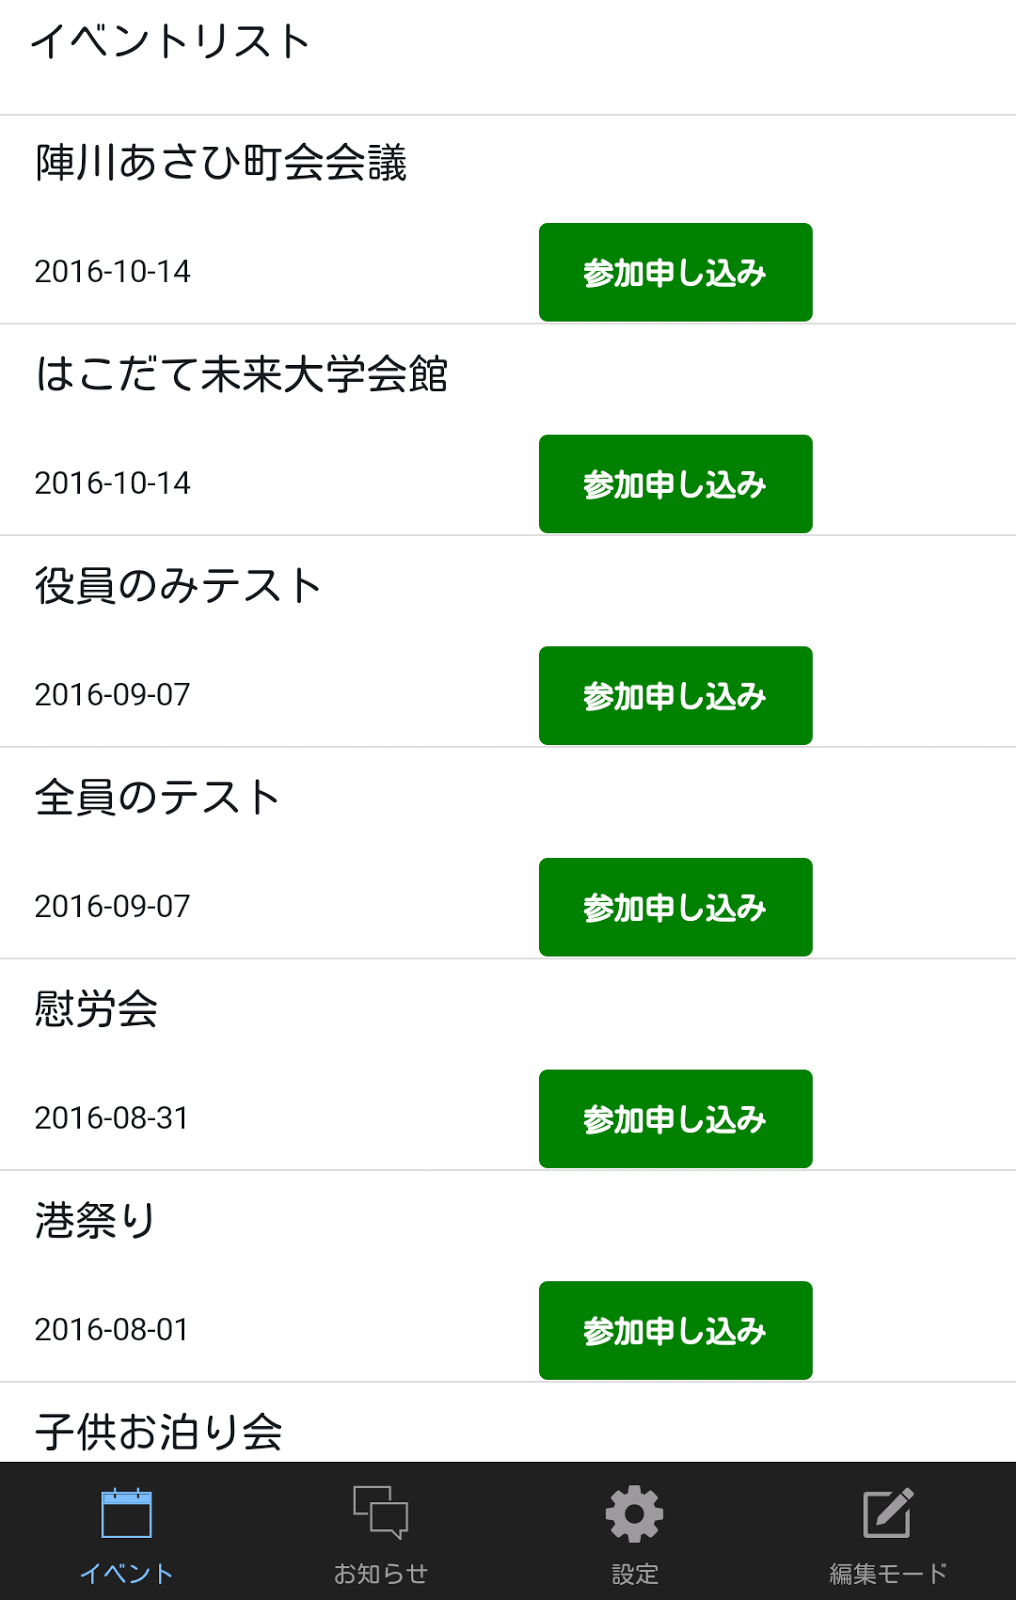
\includegraphics[keepaspectratio, scale=0.09]{picture/ui_update/beforupdate.png}
        \caption{旧イベントリスト画面}
        \label{beforeventlist}
      \end{minipage} &
      %---- 2番目の図 --------------------------
      \begin{minipage}[t]{0.3\hsize}
        \centering
        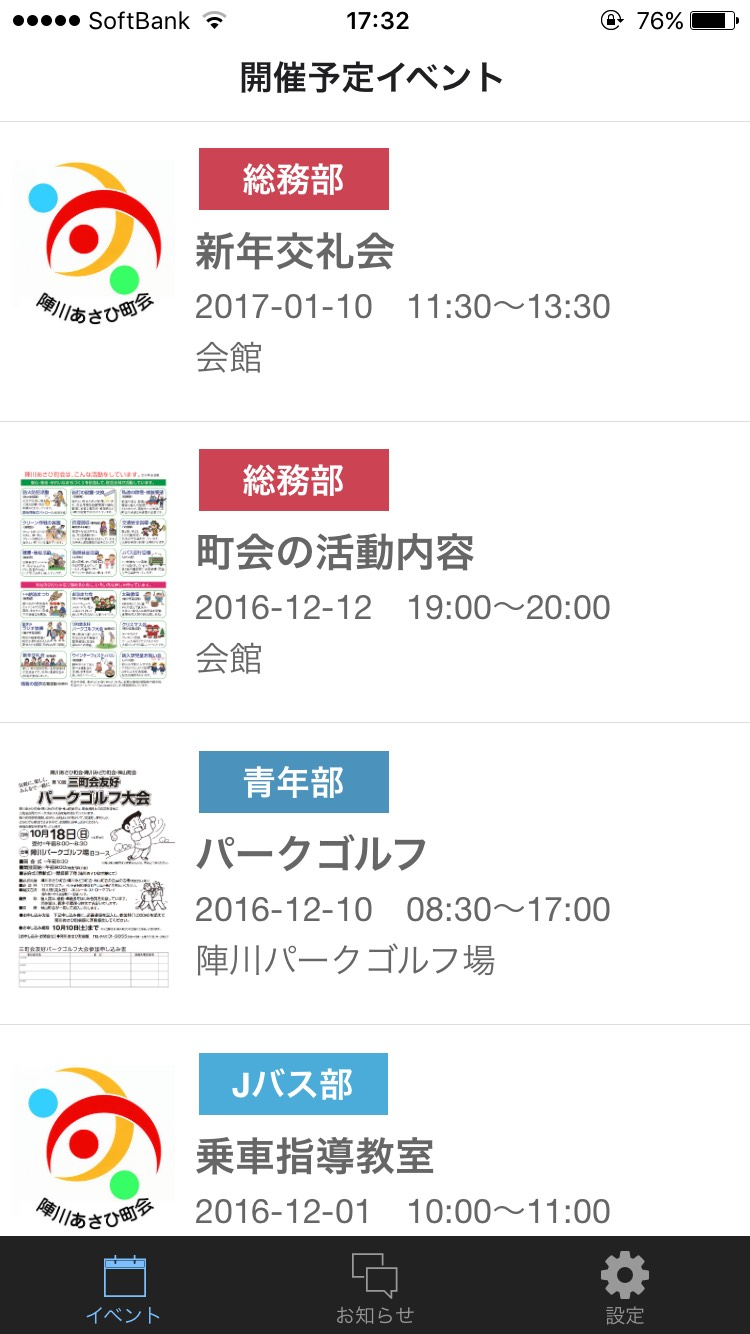
\includegraphics[keepaspectratio, scale=0.1]{picture/ui_update/afterupdate1.jpg}
        \caption{新イベント作成画面}
        \label{aftereventlist}
      \end{minipage}
      %---- 3番目の図 --------------------------
      \begin{minipage}[t]{0.3\hsize}
        \centering
        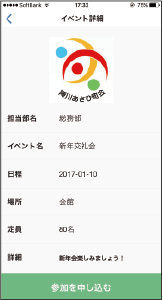
\includegraphics[keepaspectratio, scale=0.45]{picture/ui_update/afterupdate2.png}
        \caption{イベント詳細画面}
        \label{eventdetail}
      \end{minipage}
      %---- 図はここまで ----------------------
    \end{tabular}
\end{figure}

じぷりを利用する人の興味を引くためにイベントのチラシやイベントの詳細を見れるようにした.
イベントの詳細画面ではチラシをタップすると拡大表示できるようにした. 視覚的な配慮を施すために,
イベントのチラシやイベントの担当部署を色別に表示したり, イベント名の文字の大きさを変更しイベント毎の違いを明確にした.
また, 誤操作が起きないようにイベント詳細を押してからイベントへの参加申し込みをするようにした. その結果, 役員の方からはわかりやすくなり操作しやすくなったとの意見を頂いた.
\bunseki{船木綾香}

\subsection{第2回月例レビュー会}
第2回月例レビュー会で, 我々のチームは, 後期活動開始から第2回月例レビュー会までの活動の報告と, 開発途中のじぷりのデモと, 今後のスケジュールの報告を行った.
開発途中のじぷりの運用に対して, 利用しているnifty cloud mobile backendで本番運用は可能であるのか, nifty cloud mobile backendの性能の詳しい説明を先方に行うと良い,
いつから運用を開始したいのかを決めておいたほうが良いという意見を頂いた.
また, じぷりの仕様について, 参加申し込みをする際に個人の情報を毎回入力するのはとても面倒であるのでそのような手間を省くような機能を用意した方が良いという意見や,
終了したイベントは確認できないようにしたほうが良いのではという意見を頂いた.
そこで, 我々は運用に関してnifty cloud mobile backendとその他のサーバーサービスの性能を比較しメリット・デメリットを説明するための資料を作成することした.
さらに, 運用も含めた今後のプロジェクトのスケジュールを立てて, 先方に説明するための資料を作成することとした.
\bunseki{伊藤泰斗}


\section{後期第3スプリント}
\subsection{第2回集中開発}
メンバのうち2名が, 11月9日と10日に集中して開発を行った. 理由は3点ある. 1点目は, 翌週の11月18日に第5回町会打ち合わせが控えていたこと.
2点目は, 12日にアカデミックリンクが控えていたこと. 3点目は, 日々のプロジェクト学習時間の中では打ち合わせの調整や, 町会の要求の整理などグループとしての活動が多く,
アプリの開発といった個人作業を行う時間がほとんどなかったことである. また開発が進むに連れ, アプリの機能を担当するメンバとアプリのUIを担当するメンバが, 同じファイルを編集せざるを得なくなってしまい,
開発し辛い状況下にあった. この集中開発はメンバの2名が勝手にやったことである. 結果的にグループのためにはなったが, グループの予定にないこと, 仕様が定まっていない機能, 実装を前倒しした機能があり,
不要なバクの発生を招いてもおかしくはなかった. グループとして 2名には, 感謝と同時に注意をした. この2日間で実装または, 改善したした3つの機能について述べる. 1つ目は, 作成するお知らせに,
入力する情報の属性を2つ増やしたことである. 増やした2つの属性は, お知らせのタイトルと, お知らせを作成した担当部署である. 2つ目は, お知らせリスト内の作成時刻の表記の変更である.
以前から作成した各お知らせの作成時刻は表示していたが, 2016-12-23T21:47:30.587+09:00のように, ユーザには見づらい表記であったため, 2016/11/27 3:18のように見やすく改善した.
3つ目は, イベントリストとお知らせリストで, 各イベントとお知らせを作成した担当部署がはっきりわかるように, 部署ごとに色分けして着色した.
\bunseki{横山新}

\subsection{アカデミックリンク}
\subsubsection{アカデミックリンクとは}
11月12日に開催された, 函館市内8つの高等教育機関の学生や教員などの関係者による合同研究成果発表会である.
このアカデミックリンクには北海道教育大学函館校の教育学部の方や, 北海道大学水産学部の方など様々な分野の方が参加しており,
学生たちはそれぞれの研究テーマの連携や協力の可能性を探るために互いの研究について発表を行い, 交流する.
\subsubsection{発表形式}
中間発表とは異なり, プロトタイプを利用したデモンストレーションを行うのではなく、実際に開発途中のアプリでデモンストレーションを行いながら、ポスターセッション形式で我々の活動やアプリについて発表を行った.
\subsubsection{発表内容}
アプリを開発するにいたった背景や, 開発過程, アプリの概要, 今後のスケジュールの説明をアカデミックリンクの参加者に対して行った.
\subsubsection{意見・評価}
未来大の学生及び, 他大学の学生, 教員, 及び一般の参加者から様々な意見・評価を頂くことができた. 幾つかの意見・評価を以下に示す.
\begin{itemize}
    \item 函館の地域に貢献することが出来るアプリを制作しているのはとても良い
    \item 課題解決の提案をするだけでなく 実際にプロダクトを制作するのが良い
    \item 利用しているサーバに関して, 負荷耐久テストを必ず行ったほうが良い
\end{itemize}
\bunseki{伊藤泰斗}


\subsection{第5回町会打ち合わせ}
\subsubsection{目的}
\begin{enumerate}
    \item じぷりの進捗報告と完成イメージの共有
    \item nifty cloud mobile backendを運用に利用することの了承を得る
    \item 今後のスケジュールの了承を得る
\end{enumerate}

\subsubsection{手法}
\begin{enumerate}
    \item 完成イメージ図をまとめた資料を作成し, 先方へ共有した. また, 以下の
    \begin{enumerate}
        \item ログイン方法
        \item イベントの編集・参加者リストの確認・参加申し込みをするための方法
        \item 参加者リスト表示方法
        \item お知らせリスト表示方法
        \item お知らせ作成画面
    \end{enumerate}
    5つの変更点をデモを行いながら説明した.

    さらに新規で追加された以下の
    \begin{enumerate}
        \item イベント詳細閲覧機能
        \item 参加者作成・削除機能
        \item 参加者リストのcsv形式出力機能
    \end{enumerate}
    3つの機能についてもデモを行いながら説明した.

    \item 先方に運用の説明をするために作成した資料を用いながら, まず, サーバーについて概念的な説明を行った.
    その後, nifty cloud mobile backendの無償版, 有償版, その他のレンタルサーバーの性能を比較しながら説明を行い, それぞれのメリットとデメリットを提示した.
    その上でどのサービスを今後利用していくのかを町会役員の方々に決定して頂いた.

    \item 事前に作成したスケジュール説明資料を用いて, 我々が計画したスケジュールについて説明を行った. ちなみにそのスケジュールの内容は以下である.
    \begin{enumerate}
        \item 11/28 2名の役員のスマートホンににじぷりをインストールする
        \item 12/2 1部の役員のスマートホンににじぷりをインストールする
        \item 1/11~20 じぷりの完成報告とストア公開に向けた打ち合わせ
        \item 1/31 ストア公開
    \end{enumerate}
\end{enumerate}

\subsubsection{結果}
\begin{enumerate}
    \item じぷりへの新たな要望として
    \begin{itemize}
        \item 参加申し込みをする際に, 「キャンセルは町会に直接連絡してください」という1文を追加して欲しい
        \item トップページに町会の住所, 連絡先をヒョ持して欲しい
        \item 管理者を10人してパスワードを10個用意して, どの管理者が度のイベントを作成・編集したのかが確認できるようにして欲しい
        \item イベントの説明の文章が長くなったら「・・・」と省略するようにして欲しい
    \end{itemize}
    という要望をいただいた.
    \item じぷりのUIについて, 以前よりもわかりやすく, 操作しやすくなったと評価を頂いた.
    \item 運用に関して, nifty cloud mobile backend無償版の性能に納得して頂き, これからもnifty cloud mobile backendで開発を行っても良いと許可を頂いた.
    しかし, 実際に運用が始まり利用者が3000人を超えそうな場合は, 町会にサーバーを立ち上げるなど方法を考えてほしいという要望をいただいた.

    \item スケジュールに関して, 我々が提案したスケジュールに納得して頂き, 具体的な日付を決定することができた.
\end{enumerate}
\bunseki{永井陽太}

\section{後期第4スプリント}
\subsection{第6回町会打ち合わせ}
\subsubsection{目的}
2名の町会役員のスマートホンに, 実際にじぷりをインストールすることで, 役員限定公開に向けたテストを行うことを目的とした.
\subsubsection{手法}
Monacaクラウド上でじぷりをビルドし, Android用の”.apk”ファイルを入手した後, 我々のノートPCを通して2名の役員うちの1人のAndroidスマートホンにじぷりをインストールした. iOS向けにも, じぷりのビルドを行い”.
ipa”ファイルを入手しようと試みたが, Monacaクラウドの仕様上, ビルドを行うには, ”.ipa”ファイルをインストールするiPhoneのGUIDを登録した証明書を発行する必要があるので不可能であった.
\subsubsection{結果}
じぷりへの新たな要望として
\begin{itemize}
    \item イベントリストを表示する際に, 更新日も表示されるようにして欲しい
    \item イベント作成時に, 「申し込み締め切り日」を入力出来るようにして欲しい
    \item 作成日が自動で入力されて, イベント詳細確認画面で, 作成日を確認できるようにして欲しい
\end{itemize}
上記の内容が挙げられた.
また, ビルドしたじぷりの動作ついては,
町会役員のAndroidスマートホンにおいて, じぷりの起動は可能であるものの, nifty cloud mobile backendとの通信ができていないようで,
イベントリストと, お知らせリストの表示ができない状態であった. 原因は特定できておらず, 今後調査していく予定である.
\bunseki{永井陽太}

\subsection{最終成果発表}
\subsubsection{発表形式}
12/9に行われた成果発表では今後の活動に活かすことを目的とした. 成果発表会では中間発表と同様にポスターセッション形式で, ポスターを2枚作成してデモを含めて5分程度の発表を行った.
\subsubsection{発表内容}
アカデミックリンクの内容に加え, 開発プロセスについて重点をおいた説明を行った.
\subsubsection{発表方法に対する評価}
発表方法について成果発表会で得られたアンケートの「発表方法」の項目から,  発表の理解のしやすさについてのコメントを抜粋した.
\begin{itemize}
    \item 一方的に話すのではなく, 聞いている人とコミュニケーションを取りながら話せていて, 内容が頭に入ってきた.
 \item デモを含めた一連の流れが簡潔にまとめられていた.
\end{itemize}
上記のコメントより, 中間発表に比べて全員がスラスラと説明できていたことが伺える. それに加え, 「簡潔にまとめられていた」や「内容が頭に入ってきた」と評価を受けることができた. そのため中間発表の反省点を改善することができた.
\subsubsection{発表内容に対する評価}
発表内容について, 成果発表会で得られたアンケートの「発表内容」の項目から, 今後の活動内容について述べた内容についてのコメントを抜粋した.
\begin{itemize}
    \item 中間よりも使いやすくなっていたが, まだまだ見た目のが改善できそう.
    \item 家族間で扱いやすいようにすると, より良くなるいいと思った.
\end{itemize}
上記のコメントより, 中間発表に比べて使ってもらうための改善をすることが少なからずできたことが伺える. しかし全てのユーザにとって使いやすいアプリケーションの開発を目標としている中,
見た目や使い勝手に関して好評化を受けることができなかったため, 今後はより一層力をいれて取り組みたい.
また機能面についての意見をたくさん受けることもできた. 依然として開発予定であるプッシュ機能やアカウント管理機能の開発ができていないため,
これらの機能の開発が終わり次第, アンケートで受けた内容の反映をしていきたい. そうしてより多くのユーザに使われるアプリケーションにしていく.
\bunseki{伊藤泰斗}
